\documentclass{article}
\usepackage[spanish]{babel}
\usepackage[T1]{fontenc}
\usepackage[ansinew]{inputenc}
\usepackage{graphicx}
\usepackage{url}
\usepackage[numbers,sort&compress]{natbib}

\begin{document}
\title{\textbf{Movimiento Browniano}}
\author{Clara T\'ellez}
\maketitle

\section{Introducci\'on}\label{intro}

El movimiento Browniano es un fen\'omeno f\'isico en el que una
part\'icula suspendida en un fluido presenta movimiento continuo de
naturaleza aleatoria.  El bot\'anico Robert Brown fue el primero en
observarlo en 1827, pero fue Albert Einstein quien lo explic\'o en
1905 \cite{Baz}.

Al simular el movimiento Browniano se representan estos movimientos
como si se tratara de una caminata, donde la part\'icula parte de un
punto de origen y da ``pasos'' discretos (duraci\'on) de forma
aleatoria y puede hacerlo en 1 o m\'as dimensiones \cite{Eli}.  A
partir de este tipo de estudios se pueden predecir tendencias en el
comportamiento de las part\'iculas de acuerdo a las variables que se
tengan en cuenta.

El objetivo de este trabajo es examinar los efectos de la dimensi\'on
en la probabilidad de regreso al origen, as\'i como, el efecto de la
duraci\'on de la caminata en el comportamiento.

\section{Metodolog\'ia}\label{met}

Para evaluar los efectos de las dimensiones y de la duraci\'on de la
caminata en la probabilidad de regreso al origen se us\'o el paquete
estad\'istico R en su versi\'on 3.6.2.

El experimento consisti\'o en simular una caminata variando las
dimensiones entre 1 y 8 y tambi\'en los pasos de la misma como
potencias de dos con exponente de 5 a 10 en incrementos lineales de
uno.  Se realizaron 50 repeticiones para cada caso, con estos datos se
calcul\'o la probabilidad de regreso para cada una de las 8
dimensiones, as\'i mismo, se observ\'o el efecto de la duraci\'on de
la caminata sobre el comportamiento de la part\'icula.

Los datos obtenidos fueron graficados en un diagrama de cajas y
bigotes, en el que es posible visualizar, claramente, el efecto de las
dimensiones en el comportamiento de una part\'icula que presenta
movimiento Browniano.

\section{Resultados y Discusi\'on}\label{res}

Al ejecutar la simulaci\'on en R se obtuvo una matriz de datos
correspondiente a los porcentajes de regreso al punto de origen para
cada dimensi\'on y cada duraci\'on de la caminata.  En el cuadro \ref{t1} se
muestra el conjunto de datos con el que se realizar\'a el an\'alisis
de esta pr\'actica.

\begin{table} 
 \caption{Un extracto de los datos obtenidos en R; un ejemplo de la
  salida completa se encuentra en el repositorio de la tarea
  \cite{repo1}.}
 \label{t1}
 \begin{center}
 \begin{tabular}{rrr}
\texttt{pot} & \texttt{porc} & \texttt{dim} \\
  5 & 96 & 1 \\
  5 & 64 & 2 \\
  5 & 34 & 3 \\
  5 & 24 & 4 \\
  5 &  8 & 5 \\
  $\vdots$ &   $\vdots$ &   $\vdots$ \\
 10 & 72 & 2 \\
 10 & 32 & 3 \\
 10 & 20 & 4 \\
 10 & 18 & 5 \\
 10 & 20 & 6 \\
 10 &  2 & 7 \\
 10 &  6 & 8
\end{tabular}
\end{center}
\end{table}

A partir de la matriz de datos se construy\'o un diagrama de cajas de
bigotes para observar el comportamiento de una part\'icula con
movimiento Browniano (figura \ref{f1}). Cada caja corresponde a una
dimensi\'on en donde se agrupan los porcentajes de regreso al punto de
origen en las diferentes duraciones de la caminata.

La dimensi\'on afecta la probabilidad de regreso al origen, a mayor
dimensi\'on, menor probabilidad de regreso. En la caja
correspondiente a la dimensi\'on 1, los datos se distribuyen de manera
uniforme, no hay datos at\'ipicos, ni se forman bigotes, la
probabilidad de regreso est\'a muy cerca al 100\%. La caja que
representa la dimensi\'on 2 se aleja considerablemente de la caja de
la dimensi\'on 1, los datos est\'an mas dispersos en especial en el
nivel superior. La distancia que hay entre las cajas 2 y 3 es m\'as
amplia que la observada entre las cajas 1 y 2. A partir de la caja 3
se va disminuyendo la distancia entre las cajas para las dimensiones
m\'as grandes. En la caja que corresponde a la dimensi\'on 4 podemos
observar un dato at\'ipico en la parte inferior, es el \'unico dato
at\'ipico obtenido para esta matriz, por lo que estadisticamente es no
significativo. En el gr\'afico tambi\'en podemos inferir que la
duraci\'on de la caminata no afecta la probabilidad de regreso al
origen. Las cajas, en general, son uniformes y peque\~nas, lo que
evidencia que los datos se agrupan en rangos peque\~nos.

\begin{figure}
  \begin{center}
    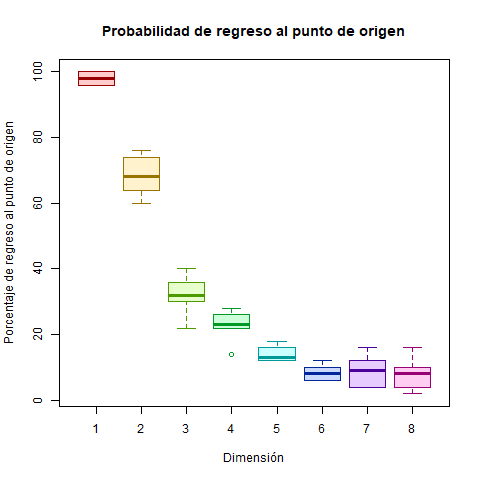
\includegraphics[width=10cm]{pr1sim.png}
  \end{center}
  \caption{Probabilidad de regreso por dimensi\'on.}
  \label{f1}
\end{figure}

\section{Conclusiones}\label{con} 
 
La dimensi\'on afecta la probabilidad de regreso al origen y la
duraci\'on de la caminata no tiene efecto sobre la probabilidad de
regreso al origen.


\bibliographystyle{plainnat}
\bibliography{simu.bib}
\end{document}
